\section{ElSe}
\label{ElSe}
Ellipse Selection for Robust Pupil Detection (ElSe), ist ein Algorithmus zur Bestimmung der Pupille in einem hochauflösenden Aufnahme des Auges unter realen Bedingungen.
\subsection{Aufbereitung der Bildinformation in der Augenregion}
\label{verbesserung_ElSe}
Zur Bestimmung der Blickrichtung ist die Augenregion natürlich von besonderer Bedeutung. Aus diesem Grund werden die Landmarks der Augenregion nochmals gesondert betrachtet. Aufgrund der besonderen Bedeutung existiert eine große Anzahl an Algorithmen, die speziell auf eine hochgenaue Bestimmung von Augenmerkmalen optimiert sind, wie Beispielsweise ElSe \cite{ElSe}, Goutam \cite{Eye_FastCorner}, Starburst \cite{Starburst}, Swirski \cite{Swirski2012}.\\
Daher bestimmt OpenFace zusätzlich zu den 64 Landmarks, die das Gesicht beschreiben, weitere 28 Landmarks pro Auge, aus denen die Blickrichtung ermittelt wird. Dazu kommt ein weiteres CLNF zum Einsatz, das auf Augen Trainiert wurde. Dabei zeigten die Vorabtests, dass die Detektionsgenauigkeit bei den getesteten kleinen Gesichtern unzureichend ausfällt.\\
Um die Position der Landmarks zu verbessern, kann auf dem Bildausschnitt der Augen der ElSe-Algotithmus eingesetzt werden. Dieser Algorithmus arbeitet auf einem Farbbild um so die Umrisse der Pupille zu berechnen. Dieses Verfahren wurde gewählt, da es im Test \cite{ElSe} am besten abgeschnitten hat und direkt das Zentrum der Pupille liefert.\\
Für die Bestimmung der Blickrichtung ist vor allem das Zentrum der Pupille und Iris sowie deren Umrisse ausschlaggebend, daher müssen diese aus dem Ergebnis von ElSe abgeleitet werden.\\
Der ElSe Algorithmus wurde für Eye-Tracking Brillen entwickelt, die die Augenregion hochauflösend abbilden. Entsprechend nimmt die Detektionsleistung bei niedriger auflösenden Bildern rasch ab und da diese Berechnung unabhängig der Landmarks ausgeführt wird, empfiehlt sich das Ergebnis zu überprüfen, damit die bestimmten Landmarks auch innerhalb der Augenhöhle liegen.\\
Bei der Berechnung wird jedes Auge unabhängig vom anderen ausgeführt. Durch die Messungenauigkeit und bei nahe an der Person befindlichen Blickzielen können die Blickrichtungen beider Augen verschieden sein. Wird ein weiter entfernterer Punkt von beiden Augen fokussiert, so kann die Blickrichtung beider Augen als parallel angenommen werden, da der unterschied zwischen Beiden minimal ausfällt. Um den Fehler zu minimieren wird als Ergebnis die durchschnittliche Blickrichtung beider Augen verwendet.
\subsection{Beschreibung}
Bei realen Aufnahmen sind Bildfehler unvermeidlich, so können Reflektionen (Brille, Kontaktlinse usw.), Make-Up und körperliche Eigenschaften wie Augenfarbe die Detektion erschweren.\\
Der Ursprüngliche ElSe-Algorithmus ist für Graubilder einer Eye-Tracking-Brille ausgelegt und optimiert. Dies betrifft vor allem die Qualität der Aufnahme im Bezug auf die Auflösung und die Infrarotbeleuchtung des Bildes, zudem ist es auf diesen Bildern zu einer Echtzeitauswertung in der Lage. Die Infrarotbeleuchtung wird verwendet, damit das Auge ausreichend beleuchtet ist ohne den Probanden zu blenden.\\
Für die Anwendung wurde ElSe angepasst um auf Farbbilder die nach Grau konvertiert wurden, arbeiten zu können. Ziel ist es die Blickrichtung möglichst exakt zu bestimmen, wofür die Landmarks der Pupille ausschlaggebend sind.\\
Als Ergebnis liefert ElSe eine Ellipse, die den Umriss der Pupille im Bild beschreibt, aus der die Landmark abgeleitet werden können.
\subsubsection{Pupille bestimmen mit Kantendetektion}
Da die Pupille als schwarzen Fleck im Bild dargestellt ist und die Iris einen helleren Farbton aufweist, wird ein Kantendetektor verwendet, der alle Pixel markiert, bei denen eine starke Farbänderung auftritt. Bei ElSe wird ein Morphologischen Ansatz eingesetzt, von Relevanz sind nur zusammenhängende Kantenpixel um die Kante zwischen Pupille und Iris zu finden, alle anderen können ignoriert werden. Wobei jedes Kantenpixel als Startpunkt der Berechnung dienen kann.\\
Um jene Kantenpixel zu erhalten, die die Pupille beschreiben, wird versucht fortlaufende Kanten zu finden, die eine Ellipse bilden. Jene die nicht diesen Anforderung entsprechen, können recht schnell ignoriert werden. Anschließend können auch alle offenen Ellipsenverläufe und jene die am meisten vom bestimmten Verlauf abweichen, verworfen werden.\\
Das beste Ergebnis aller bestimmten Ellipsen wird als Lösung verwendet.
\subsubsection{Grobe Bestimmung der Pupille}
\label{ElSe_Grob}
Sollte die Bestimmung der Ellipse, wie im letzten Kapitel beschreiben, scheitern, so wird das Zentrum des dunkelsten Kreises ermittelt. So ein Punkt kann immer gefunden werden, ist aber nicht zwingend die Pupille.\\
Auf einem verkleinertem Bild \autoref{img_else} (1) wird ein kreisförmiger Mean-Filter eingesetzt mit Ergebnis in \autoref{img_else} (3). Zur zweiten Faltung wird der Durchschnitt über ein Quadrat ohne inneren Kreis eingesetzt mit Ergebnis in \autoref{img_else} (2), wobei bei beiden Kreisen der selbe Radius verwendet wird.\\
Nun wird das Ergebnis des Quadratischen Mean-Filters invertiert \autoref{img_else} (4) und mittels Punkt-Multiplikation mit dem anderen Meanfilter zusammengebracht \autoref{img_else} (5). Im resultierendem Bild wird nun der höchste Wert gesucht, da dies das Zentrum des dunkelsten kreisförmigen Ortes im Bild ist.\\
Ergebnis des Beispiels ist als Kreuz in \autoref{img_else} (6) markiert. 
\begin{figure}
	\centering
	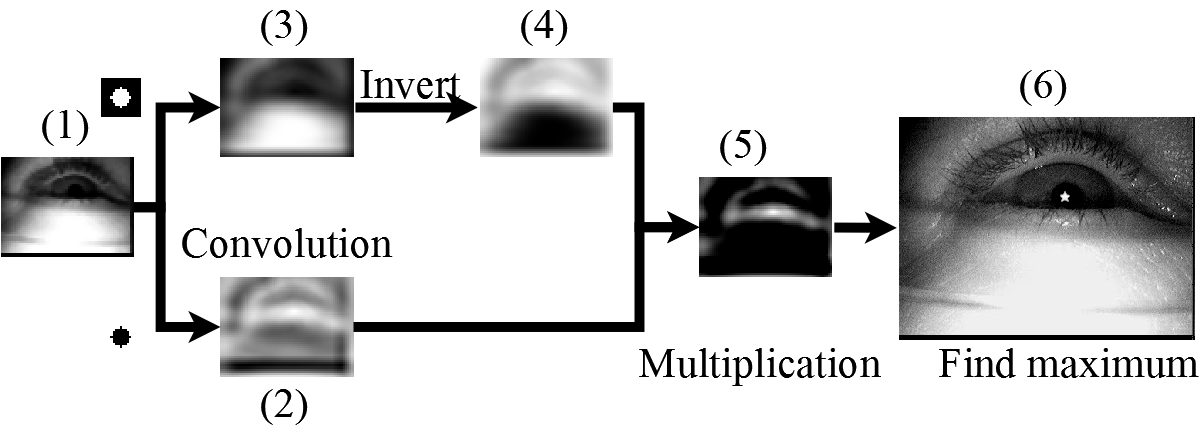
\includegraphics[width=0.8\linewidth]{img/ElSe}
	\caption{Ablauf der alternativen Berechnung zur Pupillen-Detektion von \cite{ElSe}}
	\label{img_else}
\end{figure}
\subsubsection{Ergebnisse}
Für den Test, wurden Bilder von $384\times 288$ Pixel Größe verwendet.
Im Vergleich zu den anderen Verfahren, ist ElSe in den meisten Fällen ihnen überlegen, mit einer Verbesserung der Erkennungsrate um $14.53\%$ auf dem verwendeten Datensatz \cite{ElSe}.\\
Ein Problem entsteht wenn der Farbunterschied zwischen Iris und Pupille recht gering ausfällt oder durch Reflektionen der Kantenverlauf gestört wird.\\
Für die Anwendung im aktuellen Fall, ist der Bereich der Augen sehr klein und eine eindeutige Detektion entsprechend schwierig, wodurch vor allem die grobe Bestimmung der Ellipse von Interesse ist.
\subsection{Versuchsaufbau für die Auswirkung der Graubild-Verfahren auf ElSe}
Um die einzelnen Verfahren besser Vergleichen zu können, wurden künstliche Augen aus dem Datensatz \cite{database_Eye} verwendet damit die exakte Position der Landmarks bekannt ist.\\
Ein gutes Verfahren muss stabil gegenüber der Skalierung sein, damit es auch auf kleinen Bereichen zuverlässig arbeitet. Da für die spätere Anwendung vor allem das Zentrum der Pupille von Interesse ist, wird der Abstand zum Zentrum als Qualitätsmaß verwendet.\\
Da ElSe für Eye-Tracking Brillen entwickelt wurde, also für ein Qualitativ hochwertiges Bild eines Auges, wurde der Bildbereich soweit verkleinert das noch alle Landmarks des Auges mit etwas Rand dargestellt wird, um diesen Anforderungen entsprechend nahe zu kommen.\\
Somit sind die Bildausschnitten im Datensatz auf denen gerechnet wird etwa 64 auf 29 Pixel groß und werden für die Verarbeitung auf eine Breite von 384 Pixeln vergrößert. Somit ergibt sie die Bildgröße für die ElSe entwickelt wurde, da durch die Skalierung allerdings keine zusätzlichen Informationen entstehen, ist vor allem die grobe Bestimmung der Ellipse, beschreiben in \autoref{ElSe_Grob}, von Interesse. Diese Auswahl des Bildbereiches kann auch in der späteren Anwendung eingesetzt werden, da der Augenbereich durch eigene Landmarks in der Gesichtsanalyse relativ genau bestimmt ist.\\
Um die Qualität der Berechnung bei verschiedenen Größen zu simulieren, wurde das Bild linear verkleinert.
\subsection{Auswirkung des Radius}
Ein wichtiger Parameter des ElSe-Verfahrens ist der Radius des Filters. Um den besten Parameter zu bestimmen wurde der Augen-Datensatz \cite{database_Eye} verwendet und die Augenpartie ausgeschnitten. Im Datensatz besitzen die abgebildeten Augen durchschnittlich 15 Pixel Breite Pupille und eine Iris von 34 Pixel Durchmesser.\\
In \autoref{ElSe_Gray_Iris} und \autoref{ElSe_Gray_Zentrum} ist zu erkennen, dass der Radius signifikant für die Qualität der Berechnung ist. Da für die spätere Anwendung vor allem das Zentrum der Pupille von Interesse ist, vgl. \autoref{OpenFace_Blickrichtung}, muss ElSe in diesem Aspekt zuverlässig Ergebnisse liefern.\\
Im Versuch hat sich ein Radius von etwa einem Zwölftel des zu erwartetem Durchmesser der Iris bzw. Pupille als sinnvoll erwiesen, um deren Ausmaße möglichst exakt zu bestimmen. Im Versuch entspricht dies 8 und 18 Pixel. Um die Position des Zentrums der Iris und der Pupille möglichst gut zu bestimmen, erwies sich ein Radius von 10 am besten, siehe \autoref{ElSe_Gray_Zentrum}, wobei dieser Fehler nicht so sehr steigt bei Veränderung des Radius, als bei der Größenbestimmung von Pupille und Iris.
\subsection{Auswirkung der verschiedenen Graubild-Verfahren}
Es zeigt sich das die Verfahren, um den Farbwert in einen Grauwert zu überführen, durchaus Auswirkungen auf die Qualität der Berechnung hat.\\
Das beste Ergebnis liefert das Gleab-Verfahren (Beschreiben in \autoref{gray_Gleam}) mit einer Abweichung von 5.89 Pixeln, siehe \autoref{ElSe_Gray_Zentrum}, da die Abweichung vom Zentrum minimal ist. Ein mittleres Ergebnis liefert das Luminance-Verfahren, beschreiben in \autoref{gray_Luminance}, mit welchem eine Abweichung auf dem Augen-Trainingsdatensatz von 6.42 Pixel erreicht wird.\\
Im Vergleich liefert das Quadratische-Verfahren, beschreiben in \autoref{gray_Quadrat}, die schlechtesten Ergebnis, da die durchschnittliche Abweichung bei 7.23 Pixel liegt.\\
Bei der Berechnung auf verschieden groß skalierten Bildern ist die Abweichung von ElSe bei Verwendung von Gleam konstant bei etwa 5.9 Pixel und arbeitet somit stabil, siehe \autoref{ElSe_scall}.
\begin{figure}
	\centering
	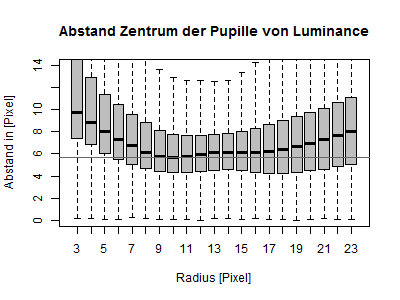
\includegraphics[width=0.32\linewidth]{Eye_Img_Box/Norm_Radius_A}
	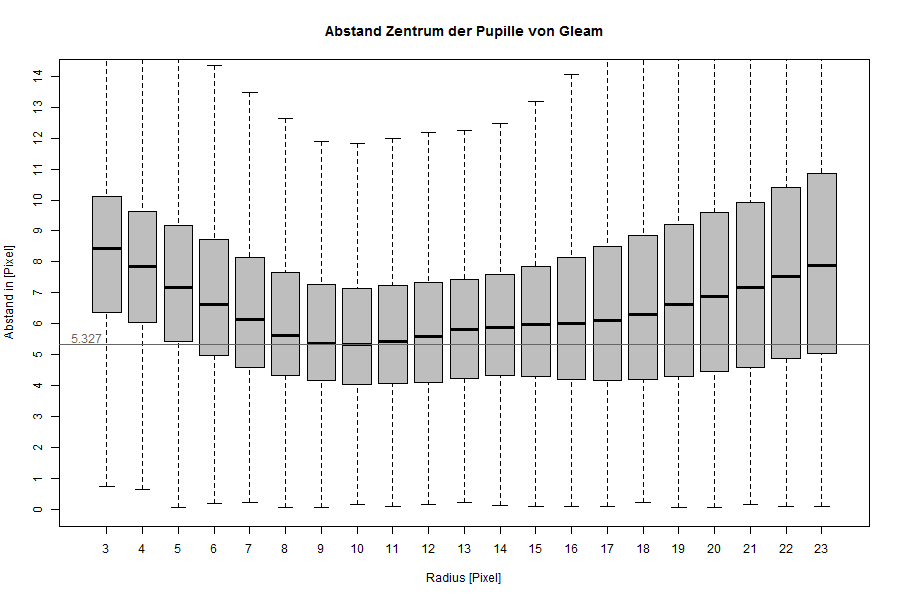
\includegraphics[width=0.32\linewidth]{Eye_Img_Box/Gleam_Radius_A}
	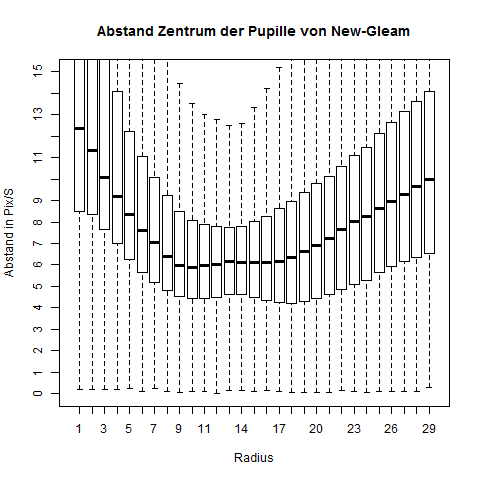
\includegraphics[width=0.32\linewidth]{Eye_Img_Box/New_Radius_A}
	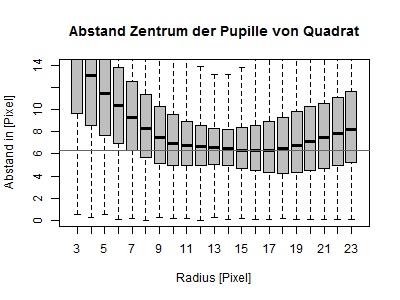
\includegraphics[width=0.32\linewidth]{Eye_Img_Box/Qua_Radius_A}
	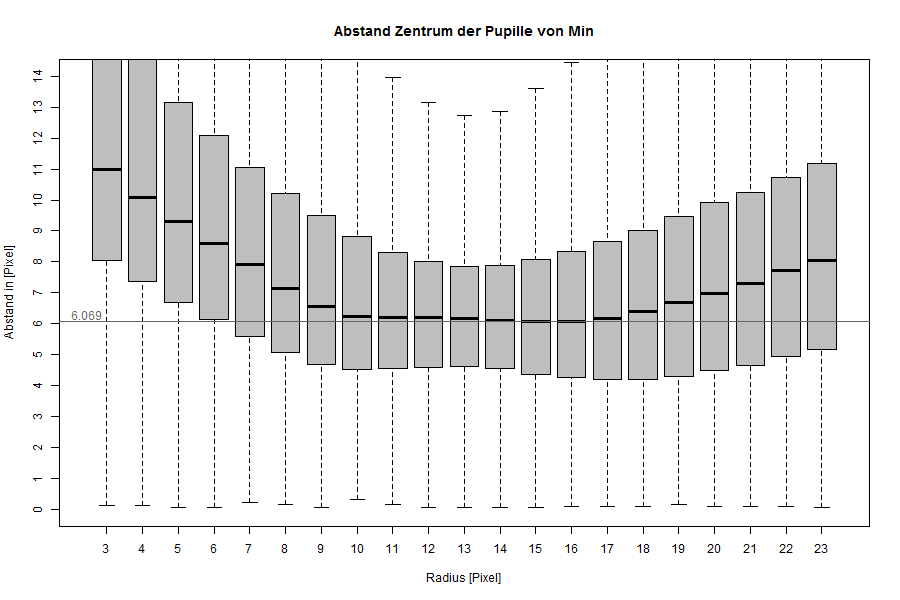
\includegraphics[width=0.32\linewidth]{Eye_Img_Box/Min_Radius_A}
	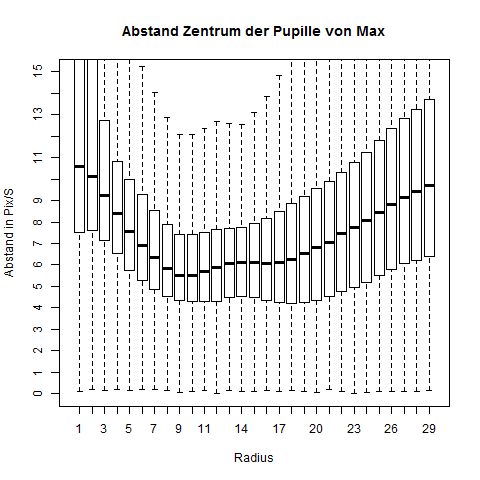
\includegraphics[width=0.32\linewidth]{Eye_Img_Box/Max_Radius_A}
	%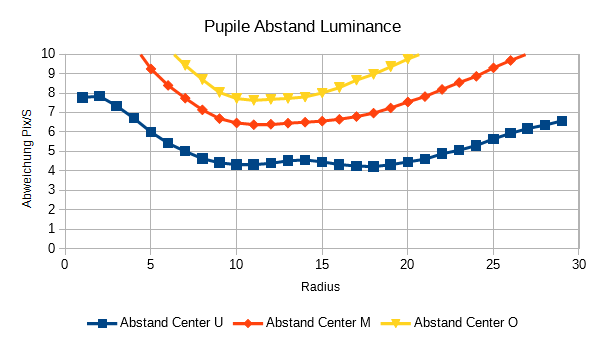
\includegraphics[width=0.49\linewidth]{Eye_Img/Normal_Abstand_P}
	%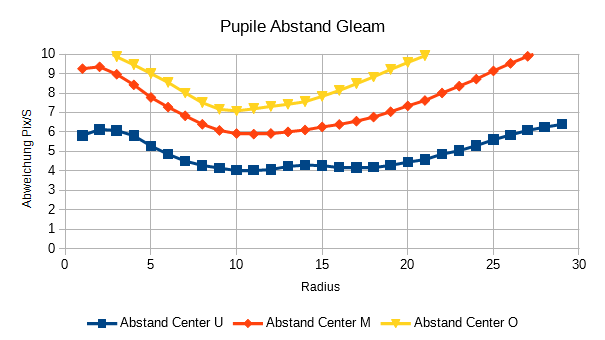
\includegraphics[width=0.49\linewidth]{Eye_Img/Gleam_Abstand_P}
	%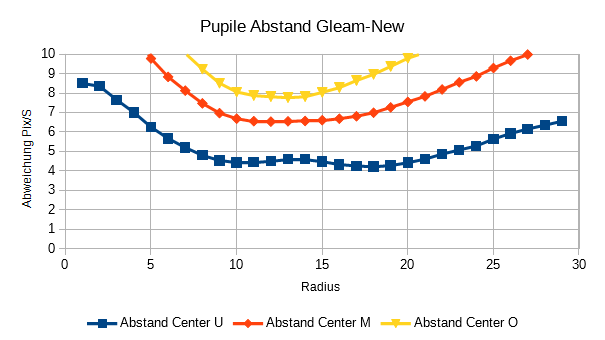
\includegraphics[width=0.49\linewidth]{Eye_Img/New_Abstand_P}
	%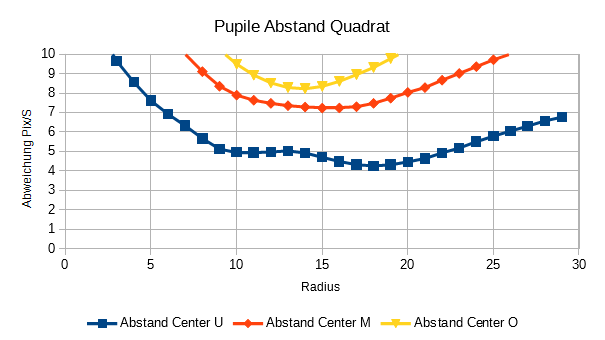
\includegraphics[width=0.49\linewidth]{Eye_Img/Quadrat_Abstand_P}
	%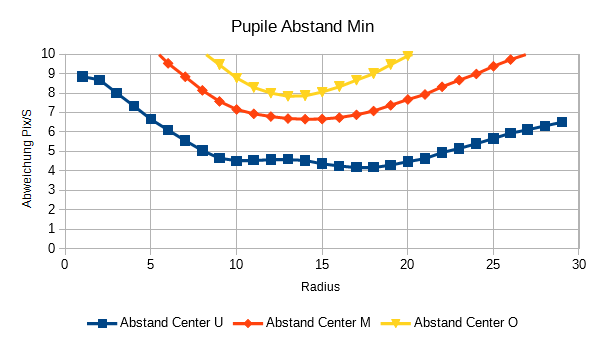
\includegraphics[width=0.49\linewidth]{Eye_Img/Min_Abstand_P}
	%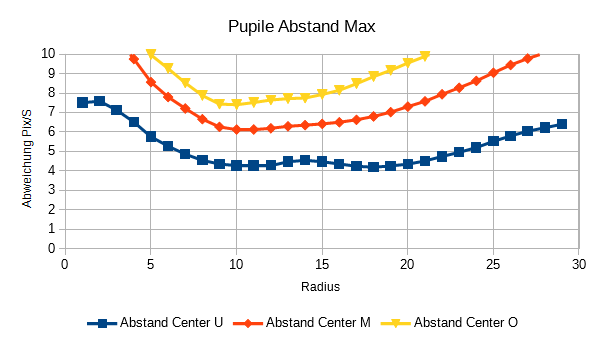
\includegraphics[width=0.49\linewidth]{Eye_Img/Max_Abstand_P}
	\caption{Abstand des Zentrums der Landmark-Pupille und der berechneten Ellipse in [Pixel/Skalierung]\\Oben-Links: Luminance, Oben-Mitte: Gleam, Oben-Rechts: Gleam New, Unten-Links: Quadrat, Unten-Mitte: Min-Wert, Unten-Rechts: Max-Wert}
	\label{ElSe_Gray_Zentrum}
\end{figure}
\begin{figure}
	\centering
	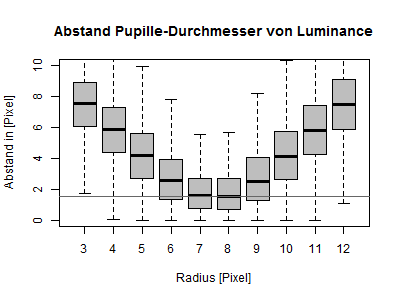
\includegraphics[width=0.32\linewidth]{Eye_Img_Box/Norm_Radius_P}
	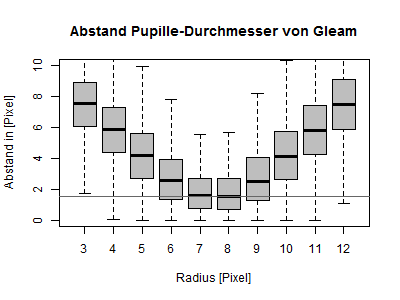
\includegraphics[width=0.32\linewidth]{Eye_Img_Box/Gleam_Radius_P}
	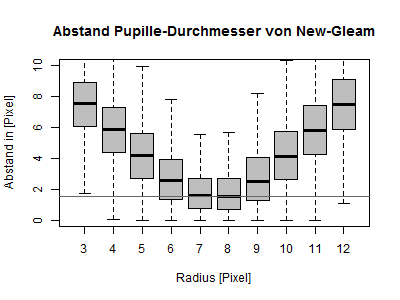
\includegraphics[width=0.32\linewidth]{Eye_Img_Box/New_Radius_P}
	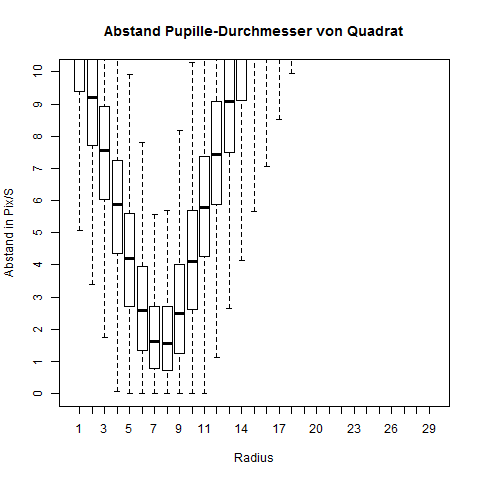
\includegraphics[width=0.32\linewidth]{Eye_Img_Box/Qua_Radius_P}
	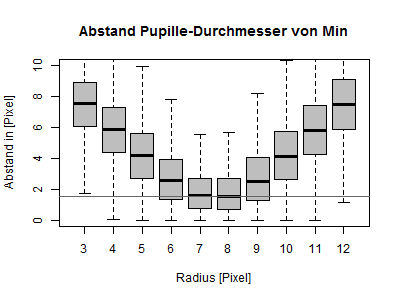
\includegraphics[width=0.32\linewidth]{Eye_Img_Box/Min_Radius_P}
	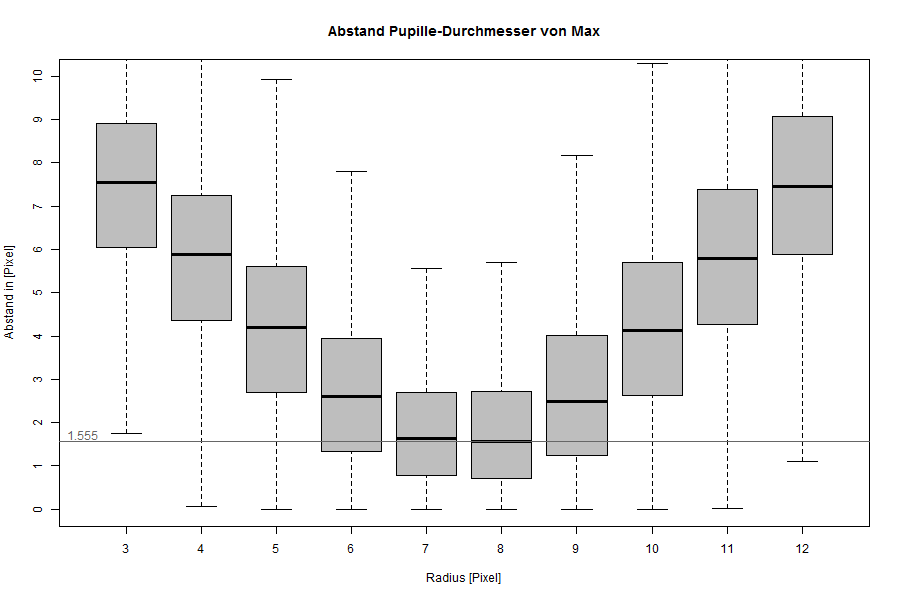
\includegraphics[width=0.32\linewidth]{Eye_Img_Box/Max_Radius_P}
	%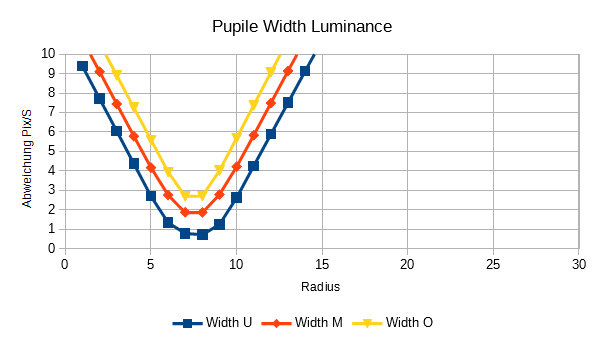
\includegraphics[width=0.49\linewidth]{Eye_Img/Normal_Width_P}
	%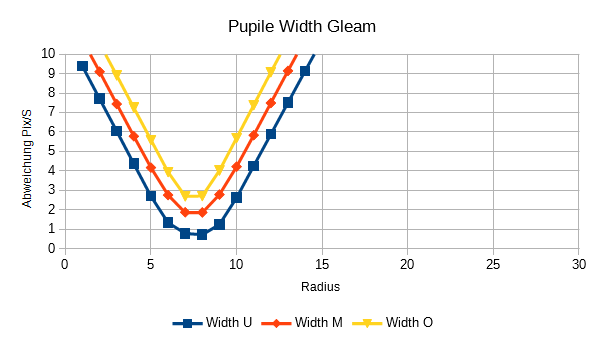
\includegraphics[width=0.49\linewidth]{Eye_Img/Gleam_Width_P}
	%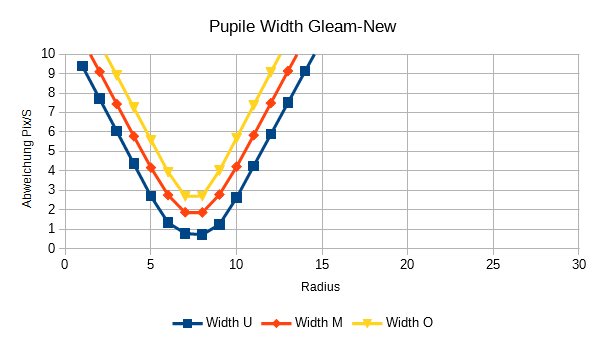
\includegraphics[width=0.49\linewidth]{Eye_Img/New_Width_P}
	%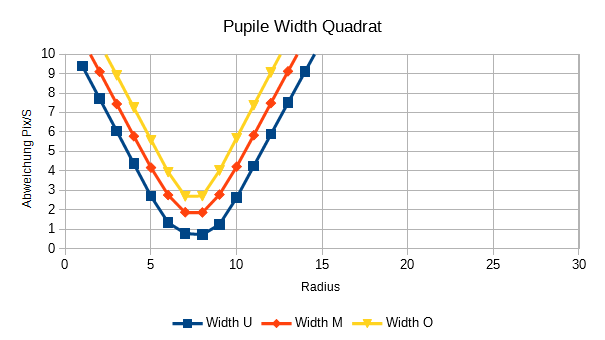
\includegraphics[width=0.49\linewidth]{Eye_Img/Quadrat_Width_P}
	%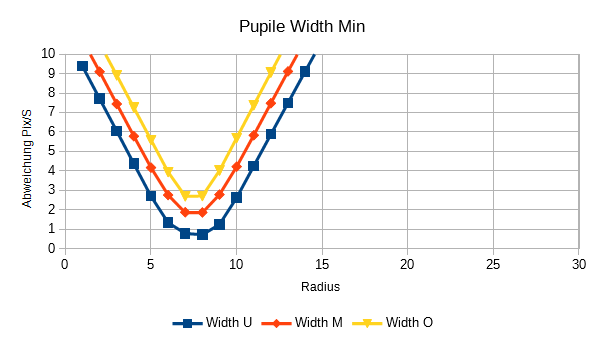
\includegraphics[width=0.49\linewidth]{Eye_Img/Min_Width_P}
	%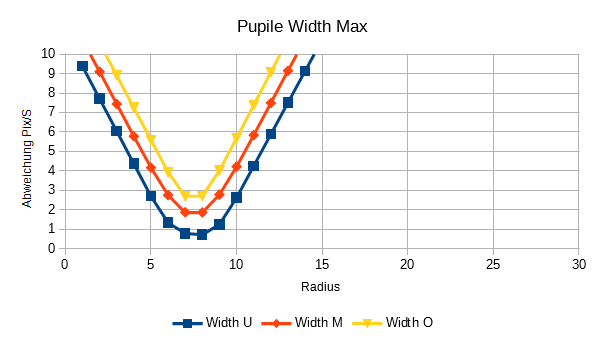
\includegraphics[width=0.49\linewidth]{Eye_Img/Max_Width_P}
	\caption{Unterschied Zwischen den Radien der Landmark-Pupille und der Berechneten Ellipse in [Pixel/Skalierung]\\Oben-Links: Luminance, Oben-Mitte: Gleam, Oben-Rechts: Gleam New, Unten-Links: Quadrat, Unten-Mitte: Min-Wert, Unten-Rechts: Max-Wert}
	\label{ElSe_Gray_Pupille}
\end{figure}
\begin{figure}
	\centering
	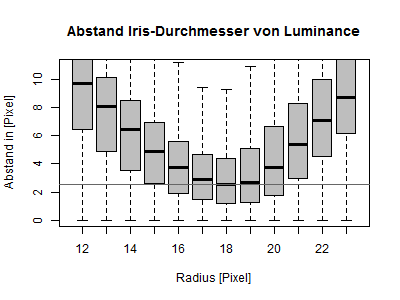
\includegraphics[width=0.32\linewidth]{Eye_Img_Box/Norm_Radius_I}
	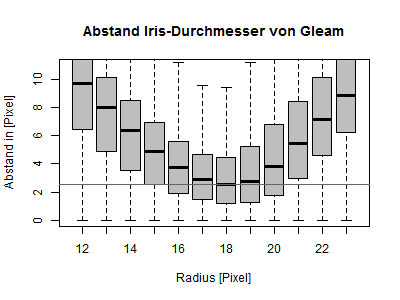
\includegraphics[width=0.32\linewidth]{Eye_Img_Box/Gleam_Radius_I}
	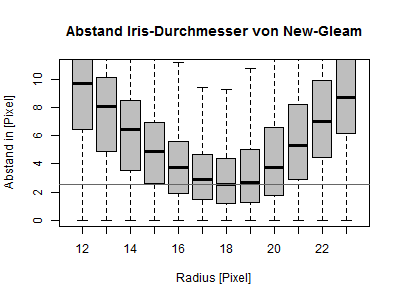
\includegraphics[width=0.32\linewidth]{Eye_Img_Box/New_Radius_I}
	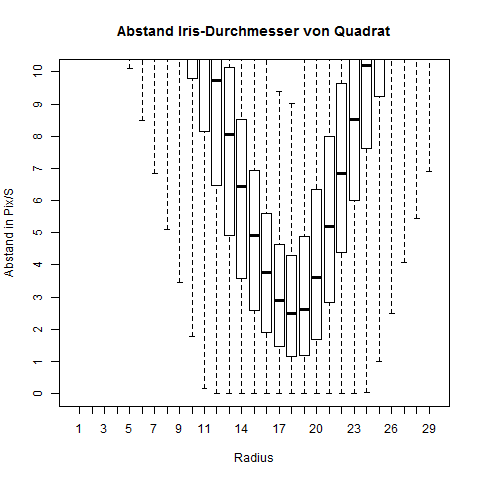
\includegraphics[width=0.32\linewidth]{Eye_Img_Box/Qua_Radius_I}
	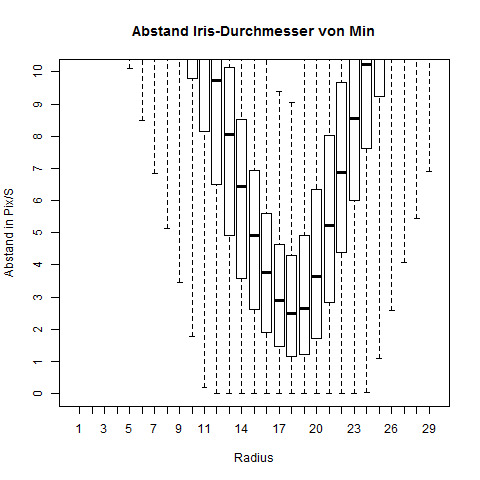
\includegraphics[width=0.32\linewidth]{Eye_Img_Box/Min_Radius_I}
	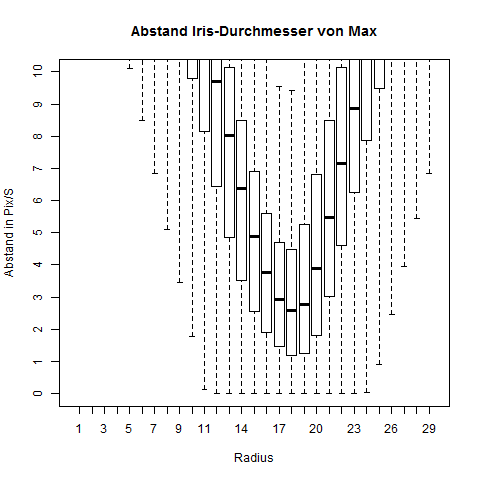
\includegraphics[width=0.32\linewidth]{Eye_Img_Box/Max_Radius_I}
	%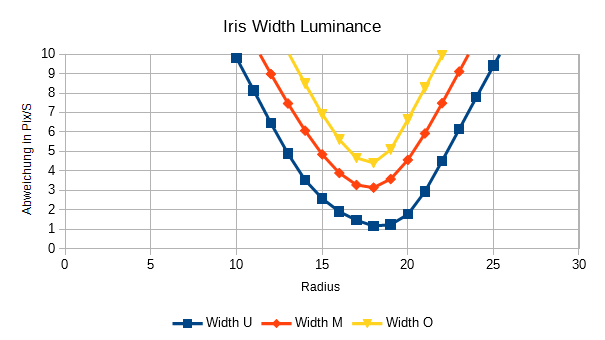
\includegraphics[width=0.49\linewidth]{Eye_Img/Normal_Width_I}
	%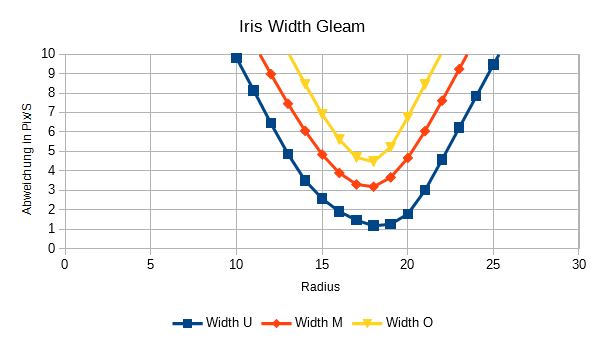
\includegraphics[width=0.49\linewidth]{Eye_Img/Gleam_Width_I}
	%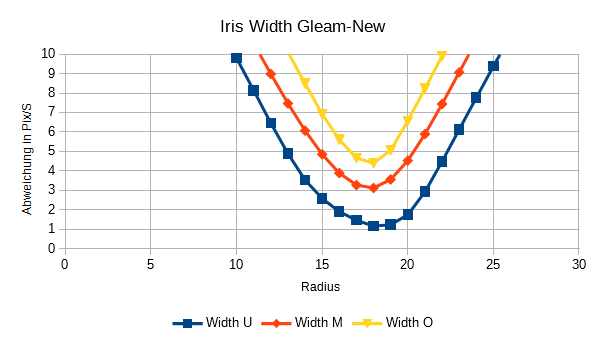
\includegraphics[width=0.49\linewidth]{Eye_Img/New_Width_I}
	%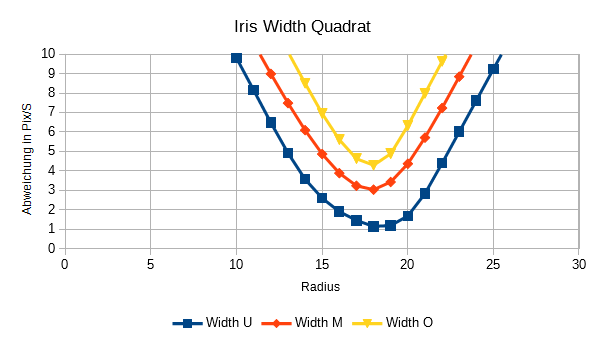
\includegraphics[width=0.49\linewidth]{Eye_Img/Quadrat_Width_I}
	%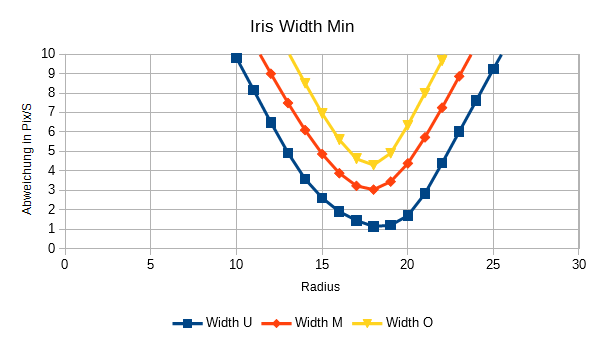
\includegraphics[width=0.49\linewidth]{Eye_Img/Min_Width_I}
	%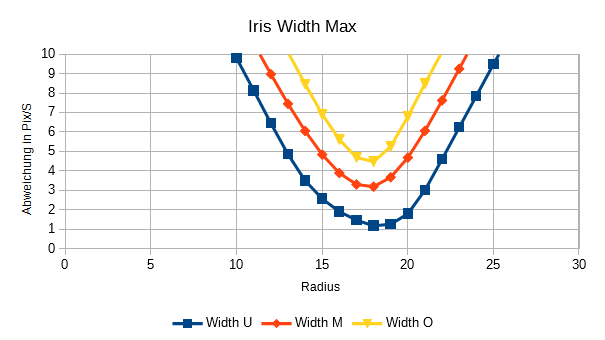
\includegraphics[width=0.49\linewidth]{Eye_Img/Max_Width_I}
	\caption{Unterschied Zwischen den Radien der Landmark-Iris und der Berechneten Ellipse in [Pixel/Skalierung] gegen die Radius-Größe.\\ Oben-Links: Luminance, Oben-Mitte: Gleam, Oben-Rechts: Gleam New, Unten-Links: Quadrat, Unten-Mitte: Min-Wert, Unten-Rechts: Max-Wert}
	\label{ElSe_Gray_Iris}
\end{figure}
\begin{figure}
	\centering
	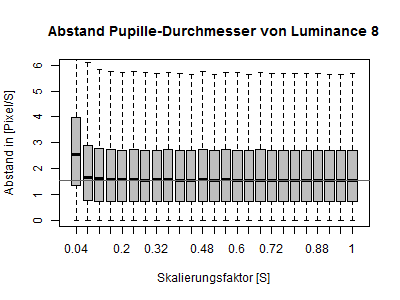
\includegraphics[width=0.32\linewidth]{Eye_Img_Box/Norm_Radius_P_8}
	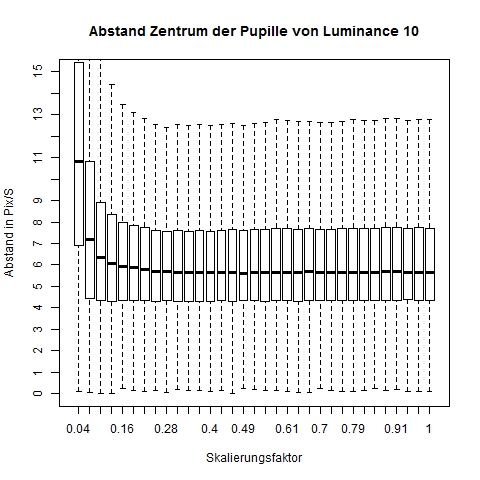
\includegraphics[width=0.32\linewidth]{Eye_Img_Box/Norm_Radius_A_10}
	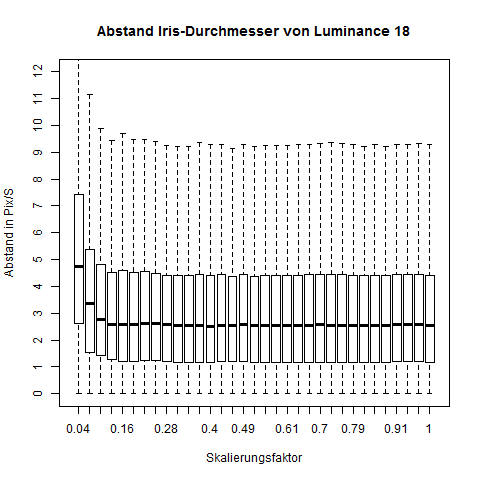
\includegraphics[width=0.32\linewidth]{Eye_Img_Box/Norm_Radius_I_18}\\
	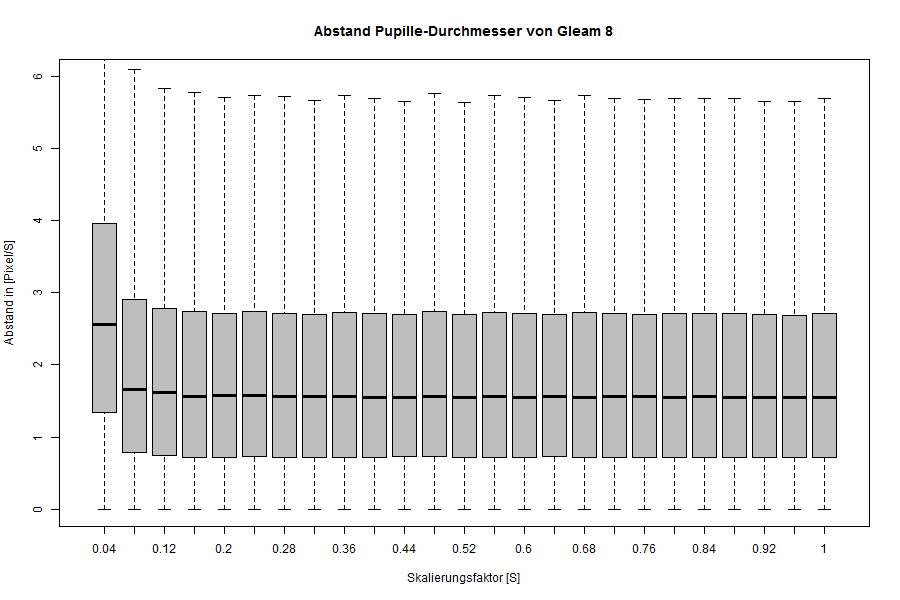
\includegraphics[width=0.32\linewidth]{Eye_Img_Box/Gleam_Radius_P_8}
	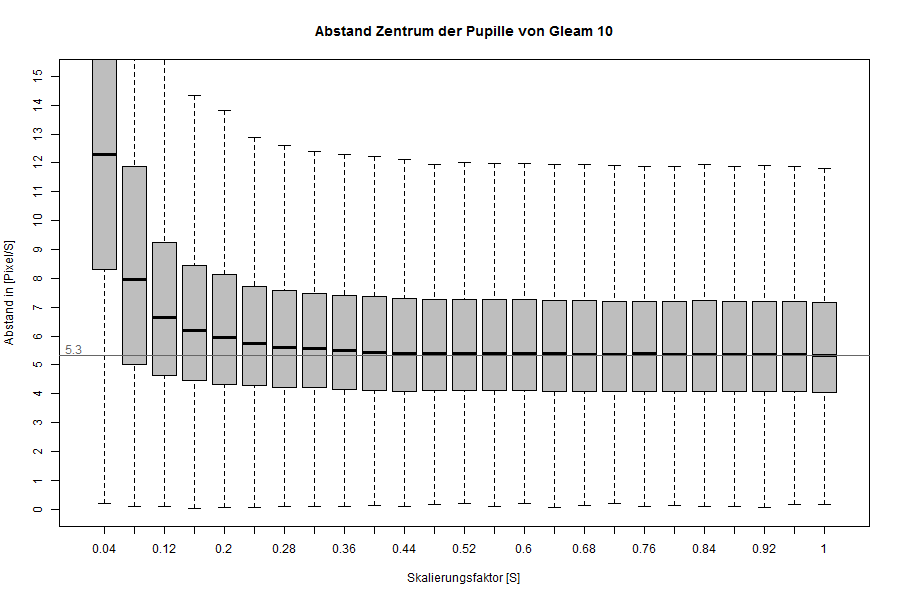
\includegraphics[width=0.32\linewidth]{Eye_Img_Box/Gleam_Radius_A_10}
	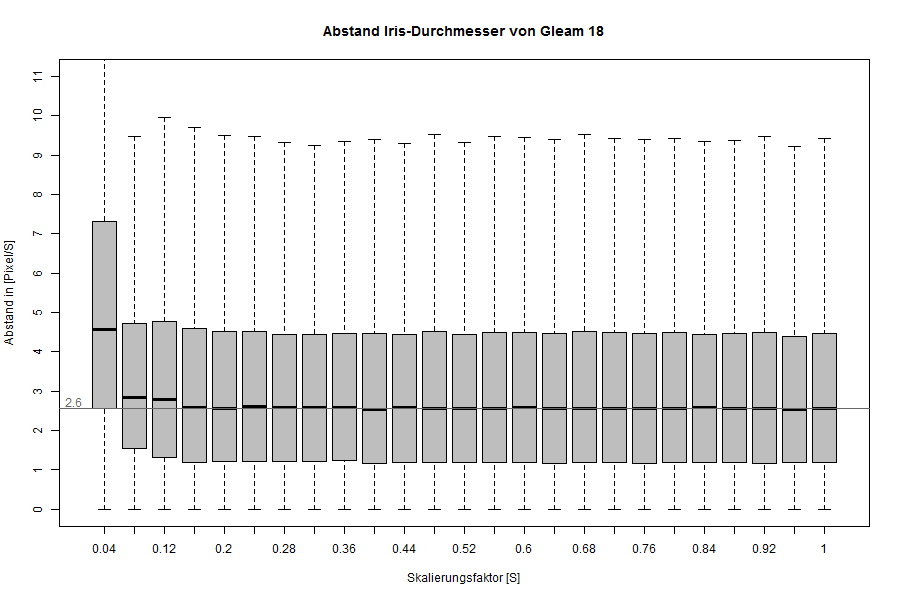
\includegraphics[width=0.32\linewidth]{Eye_Img_Box/Gleam_Radius_I_18}
	%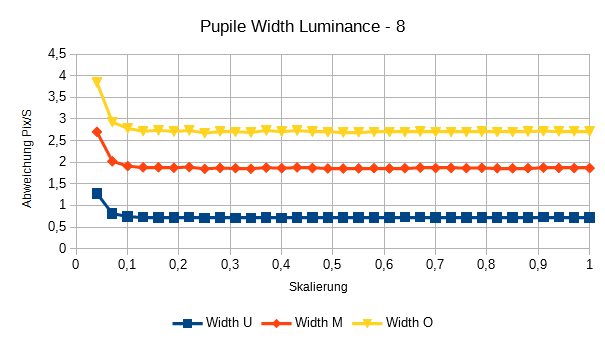
\includegraphics[width=0.32\linewidth]{Eye_Img/Normal_Width_P_8}
	%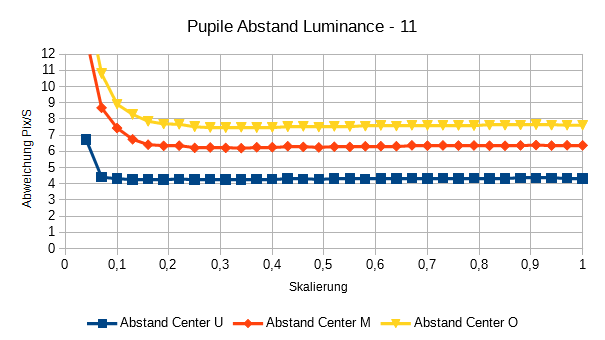
\includegraphics[width=0.32\linewidth]{Eye_Img/Normal_Abstand_P_11}
	%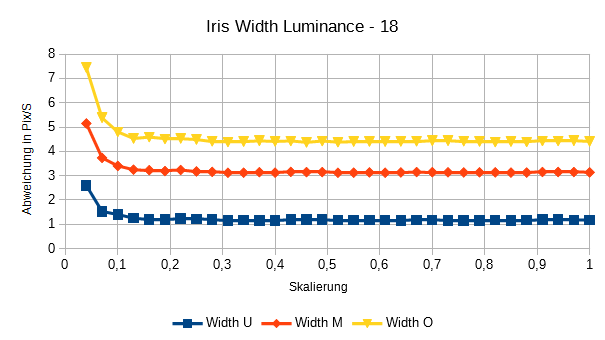
\includegraphics[width=0.32\linewidth]{Eye_Img/Normal_Width_I_18}\\
	%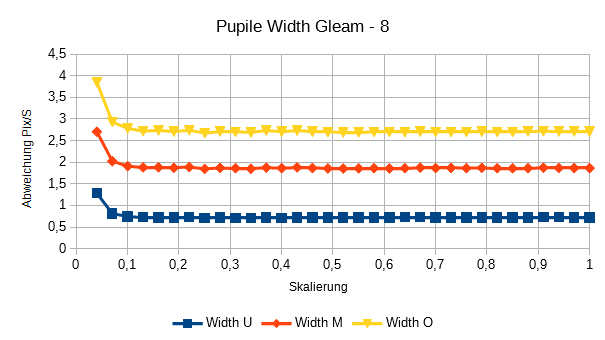
\includegraphics[width=0.32\linewidth]{Eye_Img/Gleam_Width_P_8}
	%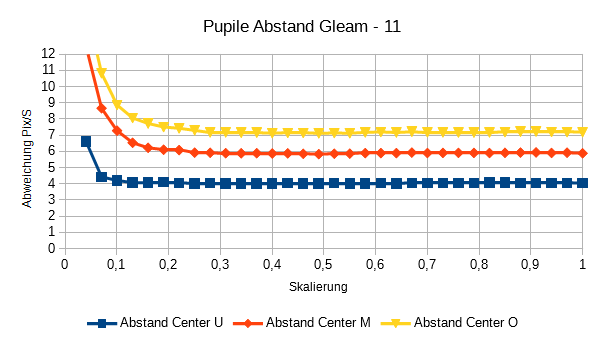
\includegraphics[width=0.32\linewidth]{Eye_Img/Gleam_Abstand_P_11}
	%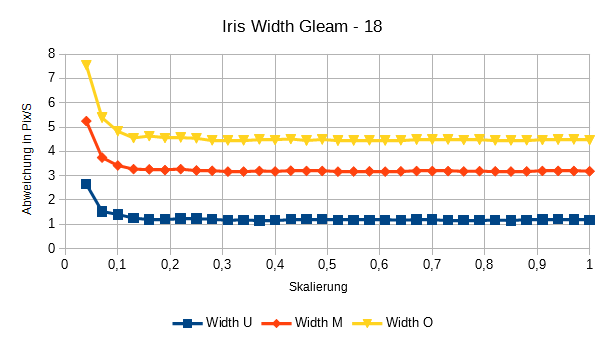
\includegraphics[width=0.32\linewidth]{Eye_Img/Gleam_Width_I_18}
	\caption{Auswirkung von der Bildgröße auf die Qualität der Berechnung.\\ Oben: Luminance, Unten Gleam}
	\label{ElSe_scall}
\end{figure}
\subsection{Vergleich zu OpenFace}
Als Referenz wird das Ergebnis von OpenFace, für die zusätzlich bestimmten Landmarks der Augen, verwendet. Dies wurde auch auf dem Augendatensatz \cite{database_Eye} angewendet um vergleichbare Ergebnisse zu erhalten.\\
In \autoref{OpenFace_Eye} ist zu erkennen dass dieses Verfahren im Schnitt oft schlechtere Ergebnisse liefert als das Ergebnis von ElSe, allerdings ohne das begehen von großen Fehlern und auch öfters genauere.\\
Da die hohe Qualität von ElSe nur erreicht werden kann, wenn es auf passenden Bildausschnitt angewendet wird, ist auch die Detektion des Auge von Interesse.\\
Nach \autoref{OpenFace_Eye_Box} ist zu entnehmen, das der Bereich des Auges zwar nicht so exakt bestimmt wird, allerdings überdeckt er den relevanten Bereich ausreichend genau. Dargestellt sind Koordinaten, X- und Y-Position in Pixel sowie die Ausdehnung der Box (Width und Hight) ebenfalls in Pixel relativ zur umschließenden Box der Landmarks. Somit liegen die Landmarks der Augen im Bildausschnitt, wodurch diese Ausschnitt verwendet werden kann als Eingabe von ElSe.
\begin{figure}
	\centering
	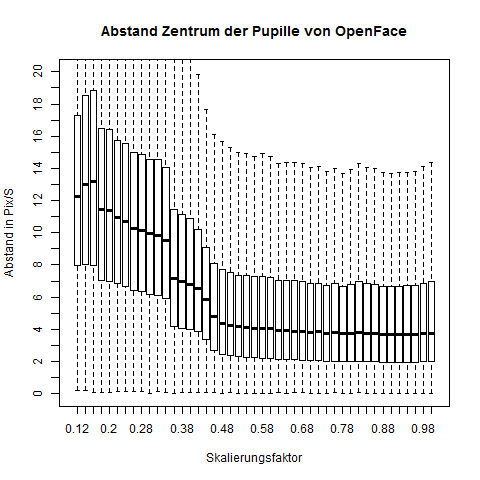
\includegraphics[width=0.45\linewidth]{Eye_Img_Box/Openface_PC}
	\includegraphics[width=0.45\linewidth]{Eye_Img_Box/Openface_PW}
	%\includegraphics[width=0.45\linewidth]{Eye_Img/OpenFace_Zentrum_P}
	%\includegraphics[width=0.45\linewidth]{Eye_Img/OpenFace_Width_P}
	\caption{Auswirkung von Skalierung auf die Qualität der Augendetektion von ObenFace}
	\label{OpenFace_Eye}
\end{figure}
\begin{figure}
	\centering
	\includegraphics[width=0.245\linewidth]{Eye_Img_Box/Openface_BoxX}
	\includegraphics[width=0.245\linewidth]{Eye_Img_Box/Openface_BoxY}
	\includegraphics[width=0.245\linewidth]{Eye_Img_Box/Openface_BoxW}
	\includegraphics[width=0.245\linewidth]{Eye_Img_Box/Openface_BoxH}
	%\includegraphics[width=0.245\linewidth]{Eye_Img/Box_X}
	%\includegraphics[width=0.245\linewidth]{Eye_Img/Box_Y}
	%\includegraphics[width=0.245\linewidth]{Eye_Img/Box_W}
	%\includegraphics[width=0.245\linewidth]{Eye_Img/Box_H}
	\caption{Bestimmung der Box ums Auge}
	\label{OpenFace_Eye_Box}
\end{figure}
\subsection{Ergebnis}
So ist im Test der Durchschnitt bei allen Skalierungen ElSe den Ergebnisse von OpenFace überlegen, durch die Verteilung ist allerdings eine Kombination beider Verfahren sinnvoll, so kann das Ergebnis von OpenFace bei Bilder in denen die Iris größer als 21 Pixel ist direkt als Lösung verwendet werden, da der mögliche Fehler von OpenFace geringer ist als von ElSe.\\
Im Bereich zwischen 21 und 15 Pixel können beide Ergebnisse Kombiniert werden, da sie ungefähr gleich gute Ergebnisse liefern.\\
Sollte die Iris im Originalbild noch kleiner sein, so ist ElSe deutlich genauer, da es noch bis zu einer Irisgröße von 3 Pixel noch stabil funktioniert.
